\chapter{Fundamentos e Revisão de Literatura}
\label{chap:fundamentacao}
É necessário definir alguns termos, técnicas e/ou ferramentas para o entendimento do trabalho. Por exemplo, a conceituação formal de sensibilidade ao contexto é muito importante, uma vez que constitue-se da técnica de obtenção dos dados. Como complemento à sensibilidade ao contexto define-se o que é o ZooKeeper, a ferramenta utilizada para transmissão dos dados coletados. Além disso, a compreensão de como o Apache Hadoop, seu escalonamento e o paradigma de programação utilizado funcionam, bem como quais trabalhos já foram feitos neste âmbito, são relevantes.

%-------------------------------------------------------------------

\section{Sensibilidade ao Contexto}
\label{sec:ctx}
Quando um usuário acessa um site por meio de um dispositivo móvel este site carrega automaticamente sua versão \emph{mobile}, a qual possui alterações que aumentam a compatibilidade com o tipo de dispositivo sendo utilizado. Uma situação semelhante ocorre quando navegadores utilizam dados de localidade para melhorar os resultados de um motor de buscas, mostrando primeiro os resultados mais relacionados com a região ou idioma do usuário. Nota-se que nas duas situações a aplicação utiliza dados específicos, o tipo do dispositivo e a localização do usuário, coletados no momento da execução e utiliza-os para adaptar o seu funcionamento de maneira a oferecer maior conforto ou usabilidade ao usuário. Estes dados representam o contexto dos usuários, o qual é definido por \cite{Dey} como qualquer informação que pode ser utilizada para caracterizar a situação de uma entidade (pessoa, lugar ou objeto) considerada relevante para a interação entre usuário e aplicação.

Sendo assim, se uma aplicação é capaz de coletar informações sobre a situação do sistema no qual está sendo executada, ela é capaz de coletar informações de contexto. Porém a simples coleta não aumenta, de fato, o desempenho desta aplicação, é necessário que ela seja capaz de responder às mudanças do ambiente detectadas. Esta capacidade de detecção e reação é caracterizada como sensibilidade ao contexto por \cite{Maamar} e vai ao encontro da definição de \cite{Baldauf} em que o sistema deve detectar mudanças e adaptar suas operações sem intervenção explícita do usuário, aumentando assim a usabilidade e eficácia da aplicação.


%-------------------------------------------------------------------

\section{Hadoop}
O \textit{framework} Apache Hadoop origina-se de outro projeto da Apache, o Apache Nutch \cite{Nutch}. O Apache Nutch iniciou em 2002 como um motor de buscas na \textit{web} de código livre , porém o projeto encontrou problemas devido a sua arquitetura. Quando a Google publicou um artigo em 2003 descrevendo a arquitetura utilizada no seu sistema de arquivos distribuídos, chamado GFS (\textit{Google File System}), os desenvolvedores do Nutch notaram que uma arquitetura semelhante resolveria seus problemas de escalabilidade. A implementação da ideia foi iniciada em 2004 e o resultado foi nomeado \textit{Nutch Distributed Filesystem} (NDFS). Contudo, a medida que o desenvolvimento do projeto ocorria o propósito original do Nutch era deixado em segundo plano, o que culminou na criação de um novo projeto em 2006. Este novo projeto foi nomeado Apache Hadoop e possui o propósito de facilitar o processamento distribuído através do paradigma do MapReduce.

\subsection{Arquitetura geral do \emph{Apache Hadoop}}
O \textit{framework} Apache Hadoop é organizado numa arquitetura de mestre-escravo e possui dois serviços principais, o serviço de armazenamento (HDFS - Hadoop Distributed File System) e o de processamento (YARN - Yet Another Resource Negotiator), os quais podem ser vistos na Figura \ref{fig:ArquiteturaHadoop}.

\begin{figure}[!ht]
\centering
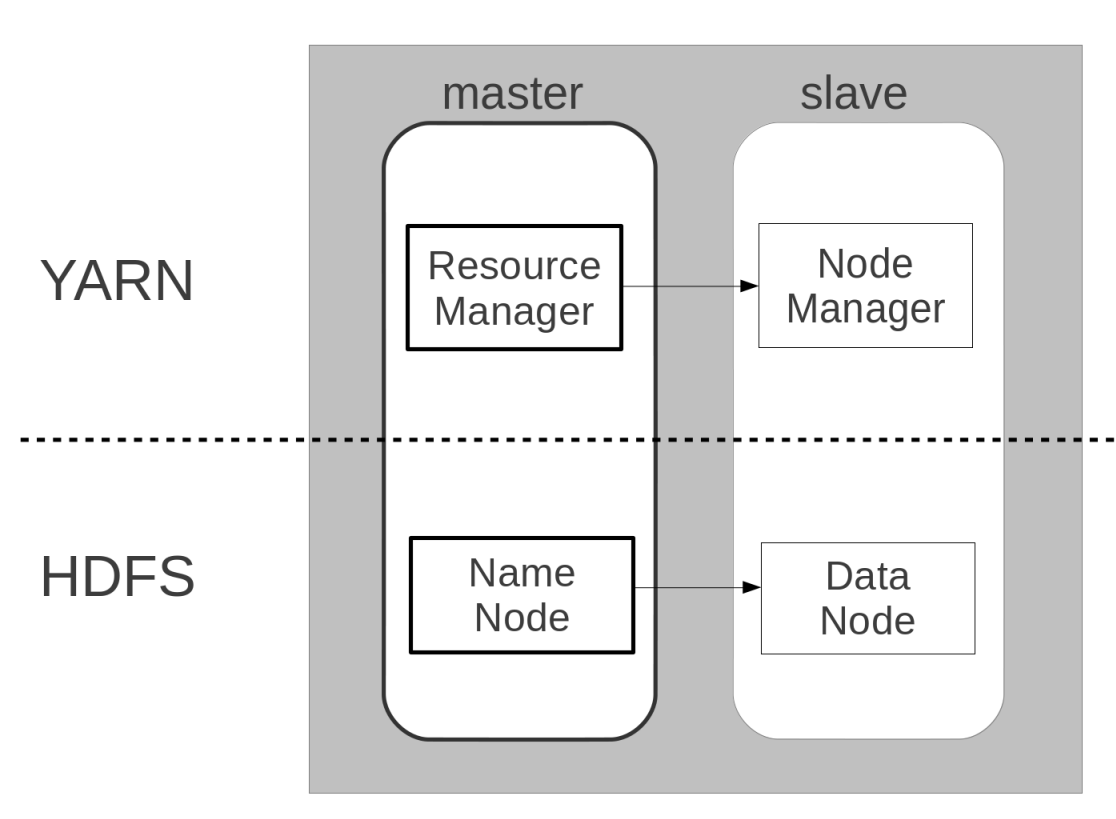
\includegraphics[width=0.7\textwidth]{figuras/Figura08-HadoooArchGeral.png}
\caption{Arquitetura geral do Apache Hadoop}
\label{fig:ArquiteturaHadoop}
\end{figure}

Nesta figura, é possível notar a existência de 4 componentes do \textit{framework}. Os componentes acima da linha pontilhada pertencem ao YARN, sendo o Resource Manager e o Node Manager os serviços mestre e escravo respectivamente. O HDFS é composto pelos componentes abaixo da linha pontilhada, sendo o Name Node e o Data Node os serviços mestre e escravo respectivamente.

\subsubsection{HDFS}
Grande parte do ganho de desempenho oferecido pelo Hadoop decorre do comportamento de levar o processamento até os dados, ou seja, todo processamento é feito com dados locais. Esta abordagem só é possível de ser realizada graças ao HDFS. Dentro do Name Node são mantidas informações de quais partes de quais arquivos estão em cada Data Node, ou seja, todos os arquivos estão divididos num grande HD distribuído e o mestre sabe exatamente qual pedaço cada escravo possui. Dessa forma cada nó executa tantos Maps ou Reduces quanto a quantidade de arquivos locais permitir, diminuindo a necessidade de utilizar a rede com transferência de arquivos e deixando-a disponível para ser utilizada para a transferência dos resultados que são os dados já reduzidos. Um problema dessa abordagem é que o Hadoop possui uma latência muito alta, sendo desaconselhável o uso do Hadoop em aplicações críticas ou de tempo real \cite{BookHadoop}. A Figura \ref{fig:ArqHDFS} apresenta um esquema básico da arquitetura do HDFS.

\begin{figure}[!hbtn]
   \centering
   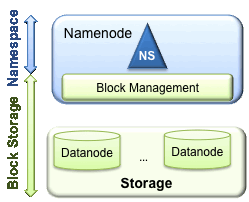
\includegraphics[width=8cm]{figuras/Figura07-HDFS.png}
   \caption{Arquitetura geral do HDFS \cite{HDFS}}
   \label{fig:ArqHDFS}
\end{figure}

\subsubsection{YARN}
Sendo o componente do Apache Hadoop responsável pela execução do \emph{MapReduce}, o YARN realiza tarefas de gerenciamento e execução do processamento. Um dos objetivos do YARN é tornar a tarefa de processamento totalmente independente das tarefas de armazenamento, possibilitando que o o \textit{cluster} seja utilizado juntamente com outras ferramentas que não utilizem o paradigma MapReduce \cite{Vavilapalli}. A Figura \ref{fig:ArqYARN} apresenta um esquema básico da arquitetura do YARN.

\begin{figure}[!hbtn]
   \centering
   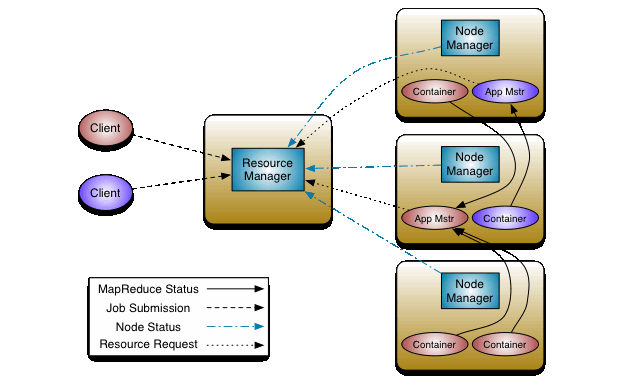
\includegraphics[width=12cm]{figuras/Figura06-YarnArch.png}
   \caption{Arquitetura geral do YARN \cite{YARN}}
   \label{fig:ArqYARN}
\end{figure}

Na imagem é possível observar dois novos componentes do YARN. O primeiro é um componente do Node Manager, possuindo o papel de um escalonador interno de cada aplicação (Application Master - referenciado na imagem como App Mstr) também conhecido por escalonador de tarefas. Considera-se que tarefas sejam uma fração do processamento das aplicações, ou seja, cada tarefa de Map ou Reduce corresponde a uma das divisões que serão processadas em paralelo. É importante não confundir este componente com o escalonador de aplicações, o qual é um componente do Resource Manager e pode ser melhor compreendido com a leitura da Seção \ref{sec:HadSched}. O outro componente presente na figura é o Container, o qual representa uma alocação de recursos em um nó qualquer do \textit{cluster}. A importância do container vem do fato de que todas as tarefas são executadas em uma instância de container.

É importante notar que existem 2 instâncias de Application Master na figura e que elas estão, assim como os clientes e os containers, coloridas de rosa ou roxo para indicar que pertencem à mesma aplicação, ou seja, o cliente rosa lançou uma aplicação que possui o Application Master e mais 3 containers de processamento. Note que o Resource manager recebe informações tanto dos clientes quanto dos Node Managers e Application Masters, centralizando todas elas para um controle dos recursos disponíveis.

\subsection{Configuração do ambiente de execução do Hadoops}
Uma característica importante do Hadoop tem relação com sua configuração. Sabe-se que todo sistema necessita de uma configuração por parte de seu administrador, e o Hadoop não é diferente com relação a isso. O Hadoop utiliza uma série de arquivos em cada um dos nós do \textit{cluster} para definir sua configuração. Estes arquivos de configuração são, na verdade, arquivos XML compostos por parâmetros de configuração e valores que influenciam o comportamento do \textit{framework} no \textit{cluster}. Para conhecimento, esses arquivos são: \emph{core-site.xml, yarn-site.xml, mapred-site.xml} e \emph{hdfs-site.xml}. Cada um destes arquivos possui propriedades de um serviço do \emph{Hadoop}, como exemplo o arquivo \emph{hdfs-site.xml} é responsável pela configuração do HDFS na máquina em questão. 

É importante salientar que para a correta execução, ao menos alguns arquivos do nó mestre devem ser configurados. No caso do administrador desejar fazer uma configuração mais específica de cada nó escravo ele deverá criar e/ou editar as propriedades nos arquivos de cada um dos nós. Caso o administrador não queira configurar os nós escravos, eles irão executar com base nos valores \textit{default}, contudo esta decisão irá, provavelmente, afetar o desempenho do \textit{cluster} devido à má configuração.

\section{MapReduce}
O paradigma de programação MapReduce é, geralmente, associado com implementações que processam e geram grandes conjuntos de dados. Neste paradigma, todo processamento é dividido em duas etapas, a etapa de Map e a de Reduce, originárias das linguagens funcionais; e todo processamento gira em torno de pares de chave e valor. Além disso, é possível de expressar uma vasta gama de tarefas reais por meio deste paradigma \cite{Dean}.

O \textit{work-flow} padrão de uma aplicação MapReduce inicia com a entrada de dados, que será dividida em \textit{n} partes e cada parte será processada individualmente por uma tarefa Map. O resultado das tarefas Map já será na forma de pares chave e valor, que serão passados como entrada para as tarefas de Reduce. Por sua vez, as tarefas de Reduce irão receber todos os pares com determinada chave e aplicar um algoritmo sobre os pares, fornecendo uma saída inteligível.

%TODO citação
A naturalidade do paralelismo deste paradigma, torna a programação da aplicação mais simples. Ao utilizar o paradigma do MapReduce o programador deve apenas pensar numa solução que siga o \textit{work-flow} do paradigma, e o parelelismo será inerente.

\section{ZooKeeper}
O ZooKeeper é um projeto da Apache e fornece ferramentas eficientes, confiáveis e tolerantes à falha para a coordenação de sistemas distribuídos \cite{Hunt2010}. Inicialmente, o ZooKeeper foi implementado como um componente do Hadoop e virou um projeto próprio conforme cresciam suas funcionalidades e sua utilização em outras aplicações. 

No caso deste trabalho, utiliza-se os serviços do ZooKeeper para monitorar e transmitir as informações de contexto coletadas nos nós escravos. No ZooKeeper existe um componente chamado \textit{znode} onde é possível inserir qualquer tipo de dado e todos as instâncias de clientes e servidores (no caso de um servidor replicado) possuem acesso à este \textit{znode}. A comunicação é feita através de processos que atualizam e processos que lêem o conteúdo destes componentes.


%-------------------------------------------------------------------

\section{Hadoop Schedulers}
\label{sec:HadSched}
Apesar de existirem dois níveis de escalonamento no Hadoop, escalonamento de aplicações e de tarefas, este trabalho possui foco somente no de aplicações. O escalonador de aplicações gerencia qual será a primeira aplicação a receber um container para seu escalonador de tarefas e quais serão os escalonadores de tarefa que receberão recursos para execução. O Hadoop já inclui alguns escalonadores que oferecem maneiras diferentes para a realização do escalonamento de aplicações. Para alterar o escalonador utilizado é necessário alterar uma propriedade no arquivo \textit{yarn-site.XML} e reiniciar o Resource Manager.

Dentre os escalonadores inclusos, o mais simples é o Hadoop Internal Scheduler que utiliza o algoritmo FIFO e tem boa performance em \textit{clusters} onde não existe competição por recursos. Este escalonador suporta até 5 níveis de prioridade, porém a decisão da próxima aplicação a ser executada sempre levará em consideração a hora de submissão.

Um pouco mais complexo que o Internal Scheduler, o Fair Scheduler é utilizado principalmente para o processamento de lotes de aplicações pequenas e rápidas, opera baseado em um escalonamento de dois níveis e possui o objetivo de realizar uma divisão justa dos recursos. O primeiro nível realiza o escalonamento na forma de filas para cada usuário ativo, dividindo os recursos do cluster igualitariamente entre as filas. Enquanto isso, o segundo nível realiza o escalonamento dentro de cada fila da mesma forma que o Internal Scheduler \cite{FairScheduler}. 

A terceira opção, e também o padrão do Hadoop nas últimas versões, é o Capacity Scheduler, o qual foi projetado para a utilização compartilhada do Hadoop e busca a maximização do \textit{throughput} e da utilização do \textit{cluster}. Seu funcionamento baseia-se em garantias mínimas de capacidade para os usuários, ou seja, qualquer usuário terá sempre uma garantia mínima de recursos para utilização. Porém quando algum usuário está com seus recursos ociosos o escalonador repassa a capacidade deste usuário  para aqueles que estão utilizando o \textit{cluster}. Esta estratégia fornece elasticidade com um bom custo benefício, uma vez que diferentes organizações possuem diferentes horários de pico para o processamento de informações. Este escalonador é capaz de rastrear os recursos registrados no Resource Manager, embora esta informação pode não ser consistente com a realidade, e monitorar quais deles estão livres e quais estão sendo utilizados pelo \textit{framework} \cite{CapacityScheduler}.

A existência destes escalonadores adiciona flexibilidade no gerenciamento do \textit{framework}. Apesar disso, os escalonadores disponíveis não detectam nem reagem à dinamicidade e heterogeneidade do ambiente. Para a utilização do Hadoop em ambientes pervasivos é necessário que exista uma capacidade de adaptação neste componente.


%-------------------------------------------------------------------

\section{Trabalhos Relacionados}
%TODO start - traduzir de volta para pt-br
%TODO revisar a parte importante dos trabalhos relacionados - no lugar de qual ctx, analisar qual o objetivo, que tipo de adaptação foi feita
%TODO adicionar os novos trabalhos que não existiam no TG
Beyond the schedulers patched together with Hadoop, there are other implementations that sought to solve a specific necessity that the standard schedulers do not offer support. A bibliographic research was made aiming to analyze the works already published involving Hadoop and having as purpose adapting or changing the scheduling. Besides, it was sought to identify which techniques were the most used and which were the most common objectives of the developed work. Following, there is a list of the related works containing a brief abstract of their proposals, used context and expected objective with the interventions.

CASH (Context Aware Scheduler for Hadoop) \cite{CASH}, this work had the objective of improving the cluster overall performance. Assuming the hypothesis that a huge part of the jobs are periodic and executed at roughly the same time, while also having similar CPU, network and disk usage characteristics. The work still takes into account that with time the nodes tend to become heterogeneous. With the intention to solve this situation, a scheduler that classifies both jobs and nodes with respect to its CPU or I/O potential was implemented, it can then distribute the jobs for machines with a more appropriated configuration regarding the job's nature.

LATE (Longest Approximation Time to End) \cite{LATE}, following what the name suggests, in this work context information is regarded to a job's estimated time to end, this time is based on a heuristic that makes the connection between elapsed time and the score. Score is a value that represents how much of the job has already been processed. This information is used to generate a threshold which will determine when a task is slow enough to start a new speculative copy on another possibly faster machine. The objective of this work was to reduce the response time in large clusters executing many jobs of short duration.

A Dynamic MapReduce Scheduler for Heterogeneous Workloads \cite{DMRSHW}, the authors of this work used the technique of classifying the jobs and machines according to the I/O and CPU potential. Just like CASH the main objective is the improvement of cluster performance. One of the differences however, is that this implementation uses a three queue scheduler.

SAMR (A Self-adaptative MapReduce) \cite{SAMR}, this implementation follow the same idea from LATE, where the context information refers to the job progress calculation and is used to identify if it is necessary to launch a speculative task. However, this solution changes a bit the calculation of progress by inserting information about the job's execution environment, the algorithm takes into account historical informations contained in each node and uses it to adjust weight of each processing step.

COSHH (A Classification and Optimization based Scheduler for Heterogeneous Hadoop Systems) \cite{COSHH}, a wider proposal if compared to the rest of the solutions, this one takes into account informations not specified about the system. It's performance gain is achieved through classification of jobs in classes, then it searches the whole cluster for machines that match the same class as the job. This search is made by an algorithm that reduces the search sample size, thus improving search response and performance. The objective of this solution is the improvement of medium job completion time, besides offering a good performance when using the minimum share and providing a fair distribution of resources.

Quincy \cite{Quincy}, this solution was not proposed solely for Hadoop environments, but still applicable to it. Possessing the objective of improving general cluster performance, uses the distribution of resources as context information and modifies the traditional way of treatment to these. In using a more dynamic approach, the solution maps the resources in a capacity-demand graph and calculates the optimum scheduling from a global cost function.

Improving MapReduce Performance through Data Placement in heterogeneous Hadoop Clusters \cite{IMRPDPHHC}, this 	solution aims to provide better performance on jobs through better data placement, using mainly the data locality as decision making information. The performance gain is achieved by the data re-balancing in nodes, leaving faster nodes with more data. This lowers the cost of speculative tasks and also of data transfers through the network.

%TODO rever o resumo final, agora será sobre os métodos e objetivos de adaptação.
After studying the related works, it is possible to note that many of them have the reduction of response time or improvement of overall performance as objective, which are slightly different from the present work that aims firstly for a better Hadoop adaptation in a heterogeneous environment, which will consequently provide a better performance.
Regarding the context, there were many contexts used although, it is possible to identify recurrent contexts such as: job classification according I/O and CPU potential, job progress evaluation in order to launch or not speculative tasks.